% !TeX program = xelatex
% !TeX encoding = UTF-8
% !TeX TXS-program:compile = txs:///xelatex | txs:///xelatex
\documentclass[aspectratio=169, table, 12pt]{beamer}

% Preamble bersama seluruh slide mata kuliah ini.
% Dipanggil dari slides/sessionXX/sessionXX.tex tepat sesudah baris
% \documentclass[aspectratio=169, table, 12pt]{beamer}
% Paket tambahan yang hanya dibutuhkan satu sesi ditulis di berkas sesi itu.

\usepackage{colortbl}
\usepackage{xcolor}
\usepackage{listings}
\usepackage{tabularx}
\usepackage{booktabs}
\usepackage{tikz}
\usepackage{pgfplots}
\usepackage{fontspec}
\usepackage[english,bahasai]{babel}
\pgfplotsset{compat=1.18}
\usetikzlibrary{arrows.meta, positioning, calc, fit, shapes.geometric,
  shapes.multipart, backgrounds, matrix, chains, trees}

\makeatletter
\def\input@path{{../theme/}}
\makeatother
\graphicspath{{../theme/}{../../figures/}}
% Stub symlink Windows memakai tema cadangan sampai aset institusi tersedia.
\IfFileExists{../theme/beamerthemePradita.sty}{%
  \usetheme{Pradita}
}{%
  \usetheme{Madrid}
  \setmainfont{TeX Gyre Heros}
  \setsansfont{TeX Gyre Heros}
  \setbeamertemplate{navigation symbols}{}
}

\definecolor{praditagreen}{RGB}{37, 113, 71}
\setbeamercolor{structure}{fg=praditagreen}
\setbeamercolor{palette primary}{bg=praditagreen,fg=white}
\setbeamercolor{palette secondary}{bg=praditagreen!80!black,fg=white}
\setbeamercolor{palette tertiary}{bg=praditagreen!60!black,fg=white}
\setbeamerfont{frametitle}{size=\large}
\setbeamertemplate{caption}[numbered]

% Ukuran header mengikuti teks agar judul panjang tidak menabrak logo.
\setbeamercolor{frametitle}{bg=white,fg=black}
\setbeamertemplate{frametitle}{%
  \begin{beamercolorbox}[wd=\paperwidth,sep=0.2cm]{frametitle}
    \begin{minipage}[c]{0.77\paperwidth}
      \raggedright\fontsize{16}{18}\selectfont\bfseries\insertframetitle
      \ifx\insertframesubtitle\empty\else
        \par\small\mdseries\insertframesubtitle
      \fi
    \end{minipage}\hfill
    \begin{minipage}[c]{0.15\paperwidth}
      \IfFileExists{../theme/classFiles/logo_universitas.png}{%
        
\includegraphics[width=\linewidth]{../theme/classFiles/logo_universitas.png}%
      }{}
    \end{minipage}
  \end{beamercolorbox}
}
\setbeamertemplate{footline}{%
  \ifnum\value{framenumber}>1
    \begin{beamercolorbox}[wd=\paperwidth,ht=0.35cm,dp=0.15cm,
      leftskip=0.3cm,rightskip=0.3cm]{palette primary}
      \footnotesize\bfseries\insertframenumber/\inserttotalframenumber
      \hfill IT40513
    \end{beamercolorbox}
  \fi
}
\DeclareRobustCommand{\berkas}[1]{\path{#1}}

% Tema membuat garis tabel berwarna putih. Dikembalikan agar tabel terbaca.
\arrayrulecolor{black}
\setlength{\arrayrulewidth}{0.5pt}

\lstdefinelanguage{yaml}{
  basicstyle=\ttfamily\scriptsize,
  keywordstyle=\color{blue}\bfseries,
  commentstyle=\color{gray}\itshape,
  stringstyle=\color{red},
  showstringspaces=false,
  breaklines=true,
  frame=lines,
  numbers=none,
  backgroundcolor=\color{lightgray!10},
  tabsize=2,
  morecomment=[l]{\#}
}

\lstdefinelanguage{json}{
  basicstyle=\ttfamily\scriptsize,
  stringstyle=\color{red},
  commentstyle=\color{gray},
  breaklines=true,
  showstringspaces=false,
  tabsize=2,
  numbers=none,
  frame=lines,
  backgroundcolor=\color{lightgray!10},
  string=[s]{"}{"}
}

\lstdefinelanguage{bash}{
  keywords={},
  basicstyle=\ttfamily\scriptsize,
  ndkeywords={docker, kubectl, helm, curl, git, terraform},
  ndkeywordstyle=\color{purple}\bfseries,
  sensitive=true,
  commentstyle=\color{gray},
  numbers=none,
  breaklines=true,
  frame=lines,
  backgroundcolor=\color{lightgray!10},
  tabsize=2,
  comment=[l]{\#},
  showstringspaces=false
}

\lstdefinelanguage{http}{
  keywords={GET, POST, PUT, PATCH, DELETE, HEAD, OPTIONS, HTTP},
  basicstyle=\ttfamily\scriptsize,
  keywordstyle=\color{blue}\bfseries,
  sensitive=true,
  numbers=none,
  breaklines=true,
  frame=lines,
  backgroundcolor=\color{lightgray!10},
  tabsize=2,
  showstringspaces=false
}

\subtitle{IT40513 · Enterprise Architecture \& Digital Blueprint}
\author{\textbf{Alfa Yohannis}}


% Sampul membatasi judul di panel putih tema rujukan Pradita.
\setbeamertemplate{title page}{%
  \begin{tikzpicture}[remember picture,overlay]
    \node[anchor=north west,inner sep=0pt,text width=8.8cm]
      at ([xshift=1cm,yshift=-3.15cm]current page.north west) {%
        {\small\insertsubtitle\par}\vspace{0.25cm}
        \resizebox{8.8cm}{!}{\begin{minipage}{12cm}
          \raggedright\color{praditagreen}\bfseries\inserttitle
        \end{minipage}}
      };
    \node[anchor=south west,inner sep=0pt]
      at ([xshift=1cm,yshift=1.65cm]current page.south west)
      {\small\insertdate};
    \node[anchor=west,inner sep=0pt,text=white]
      at ([xshift=0.8cm,yshift=0.75cm]current page.south west)
      {\small\insertauthor};
  \end{tikzpicture}
}


% Batasi kedua dimensi gambar agar diagram bersama tetap berada pada slide.
\newsavebox{\eafigbox}
\newcommand{\eadiagram}[1]{%
  \sbox{\eafigbox}{\resizebox{0.94\textwidth}{!}{\input{#1}}}%
  \ifdim\dimexpr\ht\eafigbox+\dp\eafigbox\relax>0.64\textheight
    \resizebox{!}{0.64\textheight}{\usebox{\eafigbox}}%
  \else
    \usebox{\eafigbox}%
  \fi
}


\title{\Huge Arsitektur Bisnis Saat Ini:\\ \vspace{10pt} Capability Map dan Value Stream}
\date{Pertemuan 05}

\begin{document}

\begin{frame}
  \titlepage
\end{frame}

\begin{frame}
  \frametitle{Isi Pertemuan}
  \vspace{14pt}
  \begin{columns}[t]
    \column{0.5\textwidth}
    {\small\tableofcontents[sections={1-3}]}

    \column{0.5\textwidth}
    {\small\tableofcontents[sections={4-6}]}
  \end{columns}
\end{frame}

\begin{frame}{\hfill}
  \centering
  \Huge{\textbf{Bila setiap unit punya\\bagan dan SOP, mengapa\\direksi tetap tidak tahu\\kemampuan mana yang lemah?}}
\end{frame}

\section{Tujuan dan Konteks}

\begin{frame}{\hfill}
  \centering
  \Huge{\textbf{Tujuan dan Konteks}}
\end{frame}

\begin{frame}{{\Large Tujuan Pembelajaran}}
  \vspace{10pt}
  \begin{itemize}
    \item Membedakan kapabilitas bisnis, proses bisnis, dan unit organisasi.
    \item Menyusun \textit{capability map} dua tingkat dan satu \textit{value stream} utama untuk
          organisasi \textit{capstone}.
    \item Menilai kondisi kapabilitas dalam \textit{heatmap} yang didukung bukti.
  \end{itemize}
\end{frame}

\begin{frame}{{\Large Pertanyaan Direksi Medikara Health}}
  \vspace{10pt}
  \begin{itemize}
    \item Misalkan rapat anggaran 2027: kemampuan apa yang paling menghambat strategi ``Satu
          Pasien, Satu Rekam Medis''?
    \item Bagan organisasi menjawab siapa melapor kepada siapa.
    \item SOP menjawab langkah kerja di satu tempat.
    \item Daftar permintaan menjawab apa yang ingin dibeli tiap unit.
    \item Pertanyaan direksi baru terjawab lewat kemampuan dan nilai: fase B TOGAF, luaran C2.
  \end{itemize}
\end{frame}

\begin{frame}{{\Large Diagram Konsep Bab 5}}
  \centering
  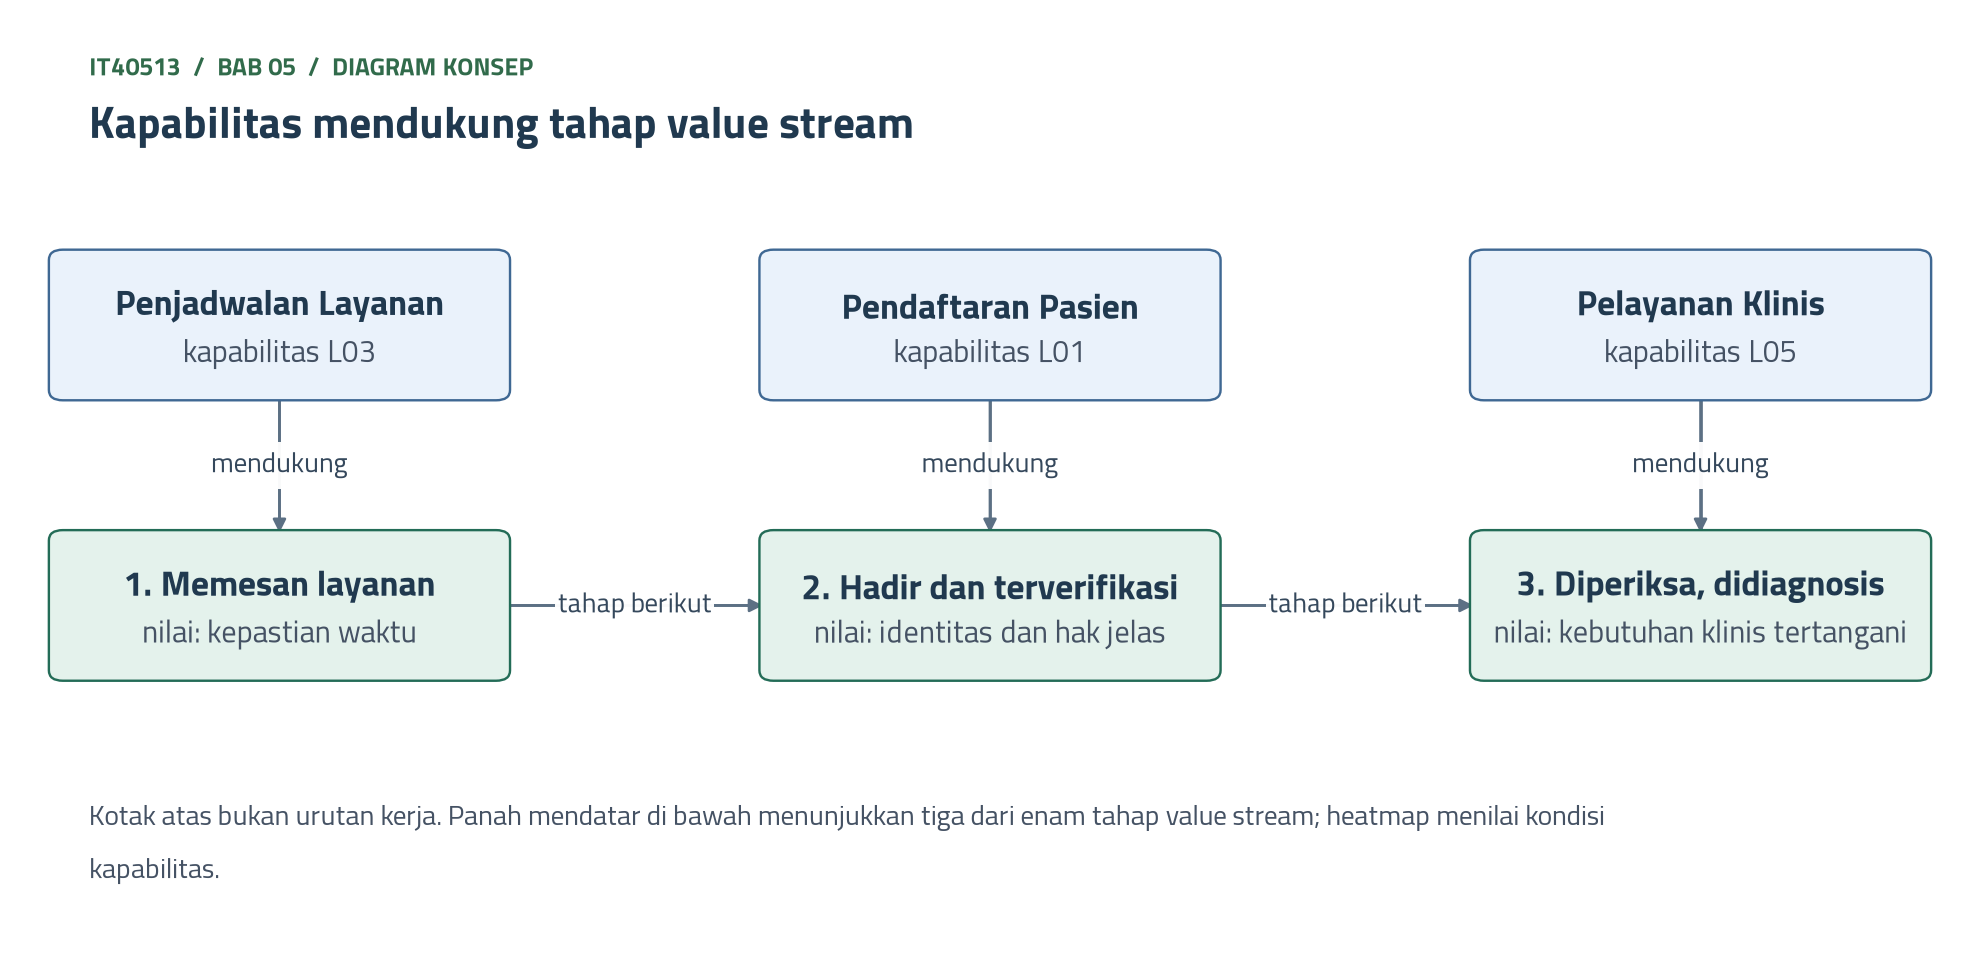
\includegraphics[width=0.96\textwidth,height=0.77\textheight,keepaspectratio]{../../figures/ch05-diagram-konsep.png}
  \label{fig:session05-ilustrasi-bab}
\end{frame}

\section{Kapabilitas dan Capability Map}

\begin{frame}{\hfill}
  \centering
  \Huge{\textbf{Kapabilitas dan\\Capability Map}}
\end{frame}

\begin{frame}{{\Large Apa Itu Kapabilitas Bisnis}}
  \vspace{10pt}
  \begin{itemize}
    \item Kemampuan yang dimiliki organisasi untuk mencapai suatu hasil.
    \item Menyatakan apa, bukan bagaimana, oleh siapa, di mana, atau dengan aplikasi apa.
    \item Diwujudkan oleh orang dan unit, proses, informasi, serta sumber daya.
    \item BIZBOK: perusahaan asuransi 100 tahun sudah punya \textit{Claims Management} sebelum ada
          otomasi.
  \end{itemize}
  \vspace{6pt}
  {\small Analogi: memasak adalah kemampuan. Mengganti kompor tidak otomatis mengajarkan
  keterampilan.}
\end{frame}

\begin{frame}{{\Large Satu Kapabilitas, Empat Unsur}}
  \centering
  \eadiagram{../../figures/ch05-kapabilitas.tex}
\end{frame}

\begin{frame}{{\Large Lima Hal yang Sering Tercampur}}
  \footnotesize
  \begin{tabularx}{\textwidth}{>{\raggedright\arraybackslash}p{2.3cm}
      >{\raggedright\arraybackslash}X >{\raggedright\arraybackslash}p{3.6cm}
      >{\raggedright\arraybackslash}p{3.3cm}}
    \hline
    \textbf{Jenis} & \textbf{Contoh Medikara} & \textbf{Pertanyaan} & \textbf{Berubah ketika} \\
    \hline
    Kapabilitas & Penjadwalan Layanan & Apa yang mampu dilakukan? & Strategi berubah \\
    \hline
    Proses bisnis & Memeriksa slot, memilih dokter, mengonfirmasi & Bagaimana pekerjaan berlangsung? & SOP direvisi \\
    \hline
    Unit organisasi & Seksi pendaftaran rumah sakit Bekasi & Siapa yang menjalankan? & Reorganisasi \\
    \hline
    Sumber daya & Medikara+, telepon, lima SIMRS & Dengan apa dijalankan? & Aplikasi diganti \\
    \hline
    Keluaran & Pesan konfirmasi jadwal & Apa hasil satu kali kerja? & Setiap proses berjalan \\
    \hline
  \end{tabularx}
\end{frame}

\begin{frame}{{\Large Contoh dan Konsekuensinya}}
  \vspace{10pt}
  \begin{itemize}
    \item 28 persen kunjungan dipesan lewat Medikara+, 72 persen lewat telepon dan loket: satu kapabilitas,
          bukan tiga.
    \item Misalkan telepon dipusatkan ke unit 40 petugas: bagan berubah, CAP-L03 tetap.
    \item Konsekuensi pertama: peta bertahan walau lima SIMRS dilebur menjadi satu.
    \item Konsekuensi kedua: 15 kapabilitas kali 8 aplikasi berarti 120 sel harus ditinjau.
  \end{itemize}
\end{frame}

\begin{frame}{{\Large Memperbaiki Nama Kapabilitas}}
  \footnotesize
  \begin{tabularx}{\textwidth}{>{\raggedright\arraybackslash}p{4.4cm}
      >{\raggedright\arraybackslash}X >{\raggedright\arraybackslash}p{4.6cm}}
    \hline
    \textbf{Nama awal} & \textbf{Masalah} & \textbf{Nama kapabilitas} \\
    \hline
    Janji temu lewat telepon & Menyebut saluran & Penjadwalan Layanan \\
    \hline
    Modul Resep SIMRS & Menyebut aplikasi & Layanan Farmasi dan Laboratorium \\
    \hline
    Bagian Klaim & Menyebut unit & Klaim dan Penjaminan \\
    \hline
    Mengisi formulir verifikasi & Langkah proses & Bagian dari Pendaftaran Pasien \\
    \hline
    Laporan bulanan direksi & Menyebut keluaran & Pelaporan Manajemen \\
    \hline
  \end{tabularx}

  \vspace{8pt}
  \small Tiap nama punya definisi satu kalimat dan kode tetap, misalnya CAP-L01.
\end{frame}

\begin{frame}{{\Large Menyusun Capability Map}}
  \vspace{10pt}
  \begin{itemize}
    \item Gambar satu halaman yang mengelompokkan seluruh kemampuan organisasi.
    \item Tingkat 1 memberi kelompok besar, tingkat 2 memberi kemampuan spesifik.
    \item Induk dan anak menyatakan penguraian, bukan urutan waktu.
    \item Tanpa panah proses: satu kapabilitas mendukung banyak proses.
    \item Kelompok membantu pembacaan, bukan menentukan prioritas.
  \end{itemize}
  \vspace{6pt}
  {\small Analogi: daftar isi perpustakaan, bukan urutan pengunjung membaca buku.}
\end{frame}

\begin{frame}{{\Large Capability Map Medikara Saat Ini}}
  \centering
  \eadiagram{../../figures/ch05-peta-kapabilitas.tex}
\end{frame}

\begin{frame}{{\Large Dari 41 Usulan dan Model Referensi}}
  \vspace{10pt}
  \begin{itemize}
    \item Misalkan 41 usulan nama: 14 aplikasi atau unit, 9 langkah proses, 3 sinonim, tersisa 15.
    \item BIZBOK bagian 8: model referensi sebagai dasar, bukan untuk disalin.
    \item Bagian 8.3 kesehatan, 8.5 asuransi, 8.6 umum, 8.8 pemerintahan.
    \item Manfaat: kemampuan yang jarang disebut dalam wawancara tidak terlewat.
    \item Risiko: menyalin kemampuan yang tidak dikerjakan organisasi.
  \end{itemize}
\end{frame}

\begin{frame}{{\Large Kasus Medikara: Tambalan dan yang Belum Ada}}
  \vspace{10pt}
  \begin{itemize}
    \item Kapabilitas tambalan: Penerbitan Nomor Rekam Medis Lokal (L02) dan Rekonsiliasi Data Manual
          Antarfasilitas (P06).
    \item Keduanya ada karena lima SIMRS tidak berbagi data.
    \item Dituntut strategi, belum ada di peta: identitas pasien lintas fasilitas, kemitraan ekosistem,
          wawasan pasien dan analitik.
    \item Yang tidak ada tidak dapat diberi warna: dicatat sebagai daftar celah C2, dibahas di Bab 8.
  \end{itemize}
\end{frame}

\section{Value Stream}

\begin{frame}{\hfill}
  \centering
  \Huge{\textbf{Value Stream}}
\end{frame}

\begin{frame}{{\Large Apa Itu Value Stream}}
  \vspace{10pt}
  \begin{itemize}
    \item Rangkaian tahap ujung ke ujung yang menghasilkan nilai bagi satu \textit{stakeholder}.
    \item Mulai dari penerima nilai, pemicu, dan nilai akhir.
    \item Satu tahap dapat melibatkan beberapa unit dan banyak proses.
    \item BIZBOK mencontohkan \textit{Settle Claim} dan \textit{Acquire Product}.
    \item Sudut pandang yang berubah mengubah batas tahap.
  \end{itemize}
  \vspace{6pt}
  {\small Analogi: pengirim paket menilai paket dijemput dan diterima, bukan penyortirannya.}
\end{frame}

\begin{frame}{{\Large Pasien Menerima Layanan Rawat Jalan}}
  \centering
  \eadiagram{../../figures/ch05-value-stream.tex}
\end{frame}

\begin{frame}{{\Large Ukuran dan Keluhan Tiap Tahap}}
  \footnotesize
  \begin{tabularx}{\textwidth}{>{\raggedright\arraybackslash}p{4.5cm}
      >{\raggedright\arraybackslash}p{3.4cm} >{\raggedright\arraybackslash}X r}
    \hline
    \textbf{Tahap} & \textbf{Nilai bagi pasien} & \textbf{Ukuran kini} & \textbf{Keluhan} \\
    \hline
    1. Memesan layanan & Kepastian waktu & Janji temu daring 28\% & 180 \\
    \hline
    2. Hadir dan terverifikasi & Identitas dan hak jelas & Median 25 menit & 640 \\
    \hline
    3. Diperiksa dan didiagnosis & Kebutuhan tertangani & Tunggu dokter 70 menit & 720 \\
    \hline
    4. Menerima obat & Obat tepat diterima & Tunggu obat 45 menit & 350 \\
    \hline
    5. Menyelesaikan pembayaran & Kewajiban biaya jelas & Klaim BPJS kembali 9\% & 190 \\
    \hline
    6. Ditindaklanjuti & Langkah berikutnya jelas & Pengingat terkirim 20\% & 70 \\
    \hline
  \end{tabularx}

  \vspace{8pt}
  \small Tahap 2 dan 3 menyumbang 1.360 dari 2.150 keluhan, sekitar 63 persen.
\end{frame}

\begin{frame}{{\Large Antrean yang Berpindah Tempat}}
  \vspace{10pt}
  \begin{itemize}
    \item Tiga waktu tunggu terbesar: $25 + 70 + 45 = 140$ menit.
    \item Misalkan dua petugas loket ditambah: tahap 2 turun menjadi 15 menit.
    \item Pasien tiba lebih cepat di ruang periksa: tunggu dokter naik menjadi 78 menit.
    \item Jumlahnya $15 + 78 + 45 = 138$ menit: perbaikan 10 menit terasa 2 menit.
    \item Ukuran ujung ke ujung dicatat di samping ukuran per tahap.
  \end{itemize}
\end{frame}

\begin{frame}{{\Large Value Stream, Proses, dan Value Stream Mapping}}
  \footnotesize
  \begin{tabularx}{\textwidth}{>{\raggedright\arraybackslash}p{2.4cm}
      >{\raggedright\arraybackslash}X >{\raggedright\arraybackslash}X
      >{\raggedright\arraybackslash}X}
    \hline
    \textbf{Aspek} & \textbf{\textit{Value stream}} & \textbf{Proses bisnis} &
      \textbf{\textit{Value stream mapping}} \\
    \hline
    Pertanyaan & Nilai apa yang diterima? & Langkah apa yang dikerjakan? & Di mana pemborosan terjadi? \\
    \hline
    Sudut pandang & Penerima nilai & Unit atau peran pelaksana & Aliran kerja satu rangkaian layanan \\
    \hline
    Rincian & Lima sampai delapan tahap & Puluhan langkah & Langkah, waktu, antrean \\
    \hline
    Di \textit{capstone} & Wajib, satu utama & Bila tahap perlu dirinci & Opsional \\
    \hline
  \end{tabularx}
\end{frame}

\begin{frame}{{\Large Kasus Medikara: Satu Kunjungan}}
  \vspace{10pt}
  \begin{itemize}
    \item Misalkan pasien lama rumah sakit Bandung berobat di rumah sakit Depok.
    \item Nomor Bandung tidak dikenali: data ditulis ulang, penjamin diperiksa ulang.
    \item Dokter memeriksa tanpa riwayat dari Bandung; resep kertas dibawa ke apotek.
    \item Menunggu 140 menit, konsultasi 15 menit: sekitar 10 persen dari 155 menit.
    \item Tahap 2 wajar bagi kepala loket, berulang bagi pasien.
  \end{itemize}
\end{frame}

\section{Pemetaan Silang dan Peta Organisasi}

\begin{frame}{\hfill}
  \centering
  \Huge{\textbf{Pemetaan Silang dan\\Peta Organisasi}}
\end{frame}

\begin{frame}{{\Large Tahap Value Stream ke Kapabilitas}}
  \centering
  \eadiagram{../../figures/ch05-pemetaan-silang.tex}
\end{frame}

\begin{frame}{{\Large Membaca Matriks}}
  \vspace{10pt}
  \begin{itemize}
    \item Pengelolaan Rekam Medis mendukung 4 dari 6 tahap: kelemahannya menjalar.
    \item Nomor rekam medis lokal muncul pada 3 tahap.
    \item Akses Pengguna adalah fondasi semua tahap, sehingga diberi tanda berbeda.
    \item Misalkan 25 menit tahap 2 terdiri atas 13 menit antre, 6 menit identitas, 6 menit penjamin.
    \item Menambah petugas hanya memperpendek antrean; layanan 12 menit per pasien tidak berubah.
  \end{itemize}
\end{frame}

\begin{frame}{{\Large Peta Organisasi: Pemilik dan Pelaksana}}
  \footnotesize
  \begin{tabularx}{\textwidth}{>{\raggedright\arraybackslash}p{5.0cm}
      >{\raggedright\arraybackslash}p{3.8cm} >{\raggedright\arraybackslash}X}
    \hline
    \textbf{Kapabilitas} & \textbf{Pemilik} & \textbf{Pelaksana} \\
    \hline
    L01 Pendaftaran Pasien & Lima kepala pendaftaran & Petugas loket 23 fasilitas \\
    \hline
    L02 Nomor Rekam Medis Lokal & Lima direktur rumah sakit & Petugas rekam medis \\
    \hline
    L04 Pengelolaan Rekam Medis & Lima kepala rekam medis & Petugas rekam medis, klinis \\
    \hline
    P01 Klaim dan Penjaminan & Kepala Klaim & Petugas loket, bagian klaim \\
    \hline
    P03 Pelaporan Manajemen & Kepala Perencanaan & Dua staf perencanaan \\
    \hline
  \end{tabularx}

  \vspace{8pt}
  \small L01, L02, L04, dan P06 tanpa satu pemilik jaringan: perbaikan harus disetujui lima orang.
\end{frame}

\section{Heatmap Berbasis Bukti}

\begin{frame}{\hfill}
  \centering
  \Huge{\textbf{Heatmap Berbasis Bukti}}
\end{frame}

\begin{frame}{{\Large Skala Kondisi Kapabilitas}}
  \footnotesize
  \begin{tabularx}{\textwidth}{>{\raggedright\arraybackslash}p{1.8cm} l
      >{\raggedright\arraybackslash}X >{\raggedright\arraybackslash}X}
    \hline
    \textbf{Skor} & \textbf{Warna} & \textbf{Ciri} & \textbf{Contoh bukti} \\
    \hline
    1 & Merah & Hasil belum konsisten, bergantung pada perorangan & Antrean, keluhan, temuan audit, sampel data \\
    \hline
    2 & Jingga & Cara kerja ada, belum merata & Ukuran hanya di sebagian fasilitas \\
    \hline
    3 & Hijau & Hasil konsisten pada lingkup yang dinilai & Ukuran stabil selama 12 bulan \\
    \hline
    Belum dinilai & Abu-abu & Data tidak tersedia & Nama pemilik dan tenggat pencarian \\
    \hline
  \end{tabularx}

  \vspace{8pt}
  \small Warna untuk satu atribut. Analogi: lampu ban dan penunjuk bahan bakar tidak dirata-ratakan.
\end{frame}

\begin{frame}{{\Large Heatmap Medikara: 4 Merah, 6 Jingga, 5 Hijau}}
  \centering
  \eadiagram{../../figures/ch05-heatmap.tex}
\end{frame}

\begin{frame}{{\Large Bukti di Balik Warna Merah}}
  \footnotesize
  \begin{tabularx}{\textwidth}{>{\raggedright\arraybackslash}p{5.6cm}
      >{\raggedright\arraybackslash}X}
    \hline
    \textbf{Kapabilitas} & \textbf{Bukti utama} \\
    \hline
    L04 Pengelolaan Rekam Medis & 1.140 dari 10.000 nomor (11,4\%), riwayat lintas fasilitas 10\% \\
    \hline
    P02 Pengelolaan Akses Pengguna & 212 akun aktif milik orang yang sudah keluar, insiden vendor 2025 \\
    \hline
    P03 Pelaporan Manajemen & Laporan terbit hari kerja ke-12, 144 hari-orang per tahun \\
    \hline
    P06 Rekonsiliasi Data Manual Antarfasilitas & 640 permintaan pencocokan per bulan, median 2 hari kerja \\
    \hline
  \end{tabularx}

  \vspace{8pt}
  \small Dua peran menilai terpisah. Data yang tidak ada ditulis belum dinilai, bukan diberi warna.
\end{frame}

\begin{frame}{{\Large Dari Warna ke Prioritas}}
  \footnotesize
  \begin{tabularx}{\textwidth}{>{\raggedright\arraybackslash}p{5.0cm} c c
      >{\raggedright\arraybackslash}X}
    \hline
    \textbf{Kapabilitas} & \textbf{Hitungan} & \textbf{Nilai} & \textbf{Ketergantungan} \\
    \hline
    L04 Pengelolaan Rekam Medis & $2 \times 3$ & 6 & Mendukung 4 dari 6 tahap \\
    \hline
    P02 Pengelolaan Akses Pengguna & $2 \times 3$ & 6 & Fondasi semua tahap \\
    \hline
    P03 Pelaporan Manajemen & $2 \times 3$ & 6 & Bergantung pada data L04 \\
    \hline
    P06 Rekonsiliasi Data Manual & $2 \times 2$ & 4 & Hilang bila data dipakai bersama \\
    \hline
  \end{tabularx}

  \vspace{8pt}
  \small Rumus hanya menyaring. Merah tidak selalu berarti diperbaiki: P06 lebih tepat dihentikan.
  Bila bobot tinggi menjadi 5, enam kapabilitas jingga bernilai 5 dan melampaui P06.
\end{frame}

\begin{frame}{{\Large Kasus Medikara: Mengapa Farmasi Hijau?}}
  \vspace{10pt}
  \begin{itemize}
    \item Layanan Farmasi dan Laboratorium hijau, padahal tunggu obat 45 menit dan 350 keluhan.
    \item Misalkan 30 dari 45 menit habis untuk resep kertas dan pencocokan data pasien.
    \item Mutu kerja apotek sendiri memenuhi ukuran internal.
    \item Akar masalah: Pengelolaan Rekam Medis dan nomor rekam medis lokal.
    \item Anggaran farmasi tidak ditambah; ketergantungan tahap 4 dicatat pada C2.
  \end{itemize}
\end{frame}

\section{Aktivitas dan Latihan}

\begin{frame}{\hfill}
  \centering
  \Huge{\textbf{Aktivitas dan Latihan}}
\end{frame}

\begin{frame}{{\Large Aktivitas: Peran dan Langkah}}
  \vspace{6pt}
  \begin{itemize}
    \item Analis bisnis memimpin penamaan kapabilitas dan tahap \textit{value stream}.
    \item Analis teknologi memeriksa dukungan sistem untuk tiap kapabilitas.
    \item Tim menyusun peta dua tingkat, satu \textit{value stream}, dan pemetaan silang.
    \item Dua peran menilai kondisi; setiap warna merah wajib berbukti angka.
    \item Pemodel memasukkan ke Archi; koordinator menjaga bukti dan kaitan dengan C1.
  \end{itemize}
  \vspace{4pt}
  {\small Data organisasi nyata seizin organisasinya, dianonimkan, tanpa data pribadi.}
\end{frame}

\begin{frame}{{\Large Luaran C2 dan Kriteria Penilaian}}
  \footnotesize
  \begin{tabularx}{\textwidth}{>{\raggedright\arraybackslash}p{4.4cm} r
      >{\raggedright\arraybackslash}X}
    \hline
    \textbf{Kriteria} & \textbf{Bobot} & \textbf{Tanda terpenuhi} \\
    \hline
    Definisi dan batas & 25\% & Definisi satu kalimat, kode tetap \\
    \hline
    \textit{Value stream} dan pemetaan & 25\% & Penerima nilai jelas, tiap tahap punya ukuran \\
    \hline
    Mutu bukti penilaian & 30\% & Merah punya angka, periode, dan sumber \\
    \hline
    Konsistensi lintas artefak & 20\% & Kode sama pada peta, \textit{heatmap}, dan Archi \\
    \hline
  \end{tabularx}

  \vspace{8pt}
  \small Luaran: \textit{capability map}, \textit{value stream}, pemetaan silang, dan \textit{heatmap},
  ditinjau menjelang UTS.
\end{frame}

\begin{frame}{{\Large Ringkasan}}
  \vspace{10pt}
  \begin{itemize}
    \item Kapabilitas menjawab apa, proses bagaimana, unit siapa, sumber daya dengan apa.
    \item \textit{Capability map} Medikara: 15 kapabilitas tingkat 2, 2 di antaranya tambalan.
    \item \textit{Value stream} rawat jalan: 6 tahap, menunggu 140 menit, 63 persen keluhan di tahap 2 dan 3.
    \item Pemetaan silang memperlihatkan akar masalah yang tersembunyi di balik gejala.
    \item Prioritas dijelaskan lewat nilai dan bukti, bukan warna semata.
  \end{itemize}
\end{frame}

\begin{frame}{{\Large Latihan}}
  \vspace{10pt}
  \begin{enumerate}
    \item Apakah ``Pendaftaran pasien di loket'' sebuah kapabilitas, proses, atau unit organisasi?
          Ubah menjadi nama kapabilitas yang tepat dan jelaskan alasannya.
    \item Susun tahapan \textit{value stream} ``Klaim asuransi dibayar'' dari sudut pandang perusahaan
          asuransi, lalu pasangkan satu kapabilitas dengan tiap tahap.
    \item Dua kapabilitas berwarna merah, tetapi anggaran hanya cukup untuk satu. Tentukan kriteria
          pemilihan dan bukti yang dibutuhkan.
  \end{enumerate}
\end{frame}

\begin{frame}{{\Large Bacaan dan Berkas Pendukung}}
  \vspace{10pt}
  \begin{itemize}
    \item \href{https://cdn.ymaws.com/www.businessarchitectureguild.org/resource/resmgr/bizbok15/BIZBOKv15_introduction.pdf}{\textit{A Guide to the Business Architecture Body of Knowledge}, Version 15}
    \item \href{https://www.opengroup.org/togaf}{\textit{The TOGAF Standard, 10th Edition}}
    \item \href{https://doi.org/10.24251/HICSS.2018.581}{Khosroshahi dkk. (2018), \textit{Business Capability Maps}}
    \item \href{https://www.lean.org/store/book/learning-to-see/}{Rother dan Shook (1999), \textit{Learning to See}}
    \item \berkas{sources/chapter05/README.md}
  \end{itemize}
\end{frame}

\end{document}
